\documentclass[11pt]{article}

\usepackage{graphicx}
\usepackage{url}

\begin{document}

\begin{titlepage}
    \begin{center}
    	
\includegraphics[scale=0.10]{du.png}\par
		\begin{Huge}
			\textsc{University of Dhaka}\par
		\end{Huge}
		\begin{Large}
            Department of Computer Science and Engineering\par \vspace{0.5cm}
            CSE-3111 : Computer Networking Lab \\[12pt]	
        \end{Large}
        \textbf{Lab Report 3:}
        Implementing File transfer using Socket Programming and HTTP
GET/POST requests \\[8pt]
        \begin{large}
            \textbf{Submitted By:\\[12pt]}
            Name: Meherun Farzana\\[8pt]
            Roll No : 05\\[12pt]
            Name: Mohd. Jamal Uddin Mallick\\[8pt]
            Roll No : 07\\[12pt]
            \textbf{Submitted On : \\[12pt]}
            February 8, 2024\\[20pt]
            \textbf{Submitted To :\\[12pt]}
            Dr. Md. Abdur Razzaque\\[12pt]
            Dr. Md. Mamun Or Rashid\\[12pt]
            Dr. Muhammad Ibrahim\\[12pt]
            Redwan Ahmed Rizvee
        \end{large}
\end{center}
\end{titlepage}

\section{Introduction}
File transfer is a critical aspect of modern networking applications, facilitating the exchange of data between systems. This lab report focuses on implementing file transfer using two essential techniques: socket programming and HTTP GET/POST requests. Socket programming provides a foundational framework for establishing communication channels between client and server applications, while HTTP protocols offer standardized methods for data exchange over the web.

\subsection{Objectives}
\begin{itemize}
    \item Develop a file transfer mechanism using socket programming to establish communication between client and server applications.
    \item Implement HTTP GET and POST requests to facilitate file retrieval and submission over the network.
    \item Evaluate the performance and scalability of the implemented file transfer system under varying network conditions and file sizes.
\end{itemize}
%%%%
%%%%
\section{Theory}
Socket programming is the foundation of network communication, facilitating the establishment of connections between client and server applications for data exchange. HTTP (Hypertext Transfer Protocol) serves as the backbone of web communication, enabling clients to request resources from servers using methods such as GET and POST. In file transfer implementations, socket programming enables connection setup and data transmission, while HTTP requests facilitate resource retrieval (GET) and data submission (POST) between client and server. Combining these techniques provides a robust framework for efficient and standardized file transfer over networks.


\section{Methodology}

\subsection{Server}
The server is initialized on a specific port and it listens for incoming requests. Whenever a client requests to connect, the server accepts the connection and provides necessary services.\\
In case of sockets, the server lets the client choose whether they want to get the list of available files, upload or download a file. The server can handle any type of file including text, audio, image, video etc. of all formats.\\
In case of HTTP, the server is an HTTP server, serving GET and POST requests from clients.

\subsection{Client}
The client side is a program requesting service from the server. It tries to connect to the server address mentioning the particular port on which the server is serving. When the server accepts the connection, it is provided with the options of service the client can avail. The client selects whether they want to see the list of available files, upload or download a file.\\
In case of HTTP, the client can make a \emph{GET} request to the server for a specific resource and avail it. Also it can make a \emph{POST} request for uploading new files into the server.

\section{Experimental result}

Some Snapshots of the Client Side queries can be seen in the following figures: 
\begin{figure}[!h]
\centering
% 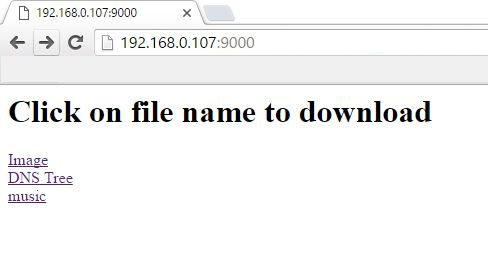
\includegraphics[width=\textwidth]{Request.JPG}
\caption{Content of Server}
\end{figure}

\begin{figure}[!h]
\centering
% 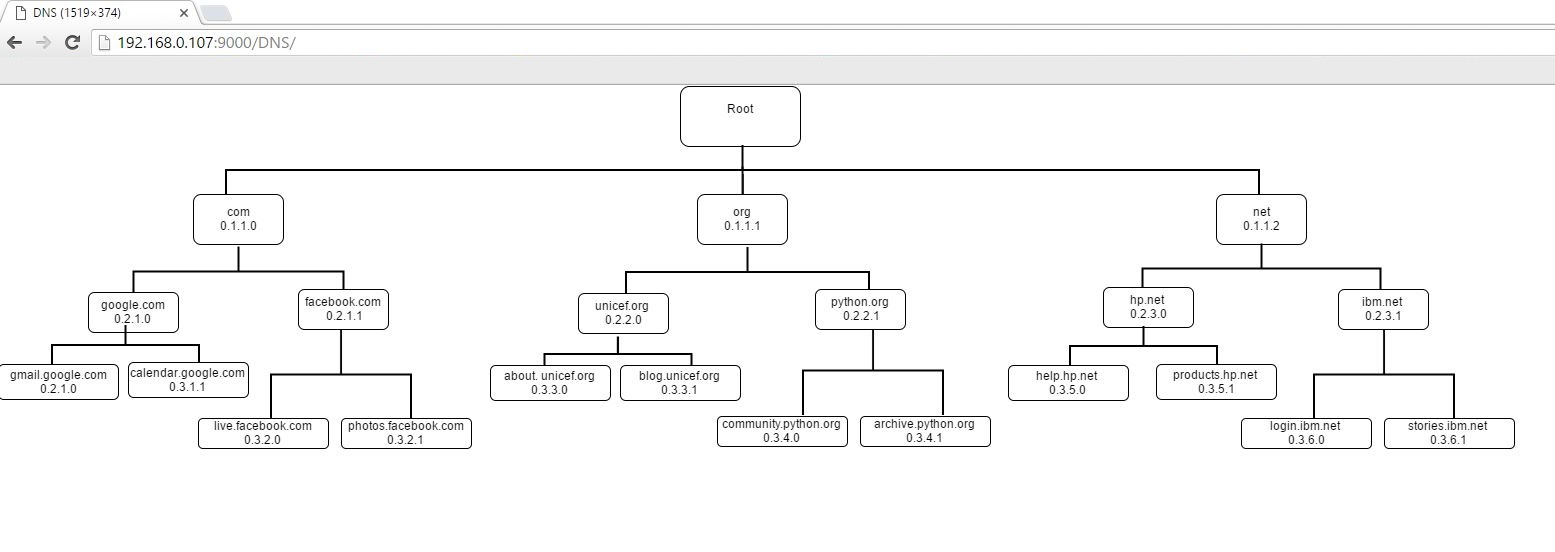
\includegraphics[width=\textwidth]{Result.JPG}
\caption{Client Side View after successful request}
\end{figure}


\newpage
\section{Experience}
\begin{enumerate}
\item We had to learn how to enable the server to handle multiple client at once.
\item We had to see some examples of how to use HttpServer package in Python
\end{enumerate}


\bibliographystyle{plain}
\bibliography{ref} % Assuming your BibTeX file is named "ref.bib"
\nocite{*}


\end{document}
